% !TeX spellcheck = en_GB
%%%%%%%%%%%%%%%%%%%%%%%%%%%%%%%%%%%%%%%%%%%%%%%%%%%%%%%%%%%%%%%%%%%%%%%%%%%%%%%%
%\documentclass[handout]{beamer}\mode<handout>{\usetheme{default}}
%
%\documentclass[presentation]{beamer}\mode<presentation>{\usetheme{blackAMSBolognaFC}}
\documentclass[handout]{beamer}\mode<handout>{\usetheme{AMSBolognaFC}}
% \setbeamertemplate{bibliography item}{\insertbiblabel}
%%%%%%%%%%%%%%%%%%%%%%%%%%%%%%%%%%%%%%%%%%%%%%%%%%%%%%%%%%%%%%%%%%%%%%%%%%%%%%%%
\usepackage[english]{babel}
\usepackage[utf8]{inputenc}
%
\usepackage{magnini-ecai-2025-talk}
%%%%%%%%%%%%%%%%%%%%%%%%%%%%%%%%%%%%%%%%%%%%%%%%%%%%%%%%%%%%%%%%%%%%%%%%%%%%%%%%
\title[Learning \EL Terminologies from LLMs]{
    % same title of the presented paper
    Actively Learning \EL Terminologies
    \\
    from Large Language Models
}
%
% \subtitle{Extended Abstract}
%
% same authors order of the presented paper
\author[Magnini et al.]{
	\emph{Matteo Magnini}$^{*}$ % empth the presenting author
	\and 
	Riccardo Squarcialupi$^{*}$
	\\
	Martin T. Sterri$^{\dagger}$
	\and
	Ana Ozaki$^{\dagger,\ddagger}$
}
%
\institute[UniBo, Uni*]{
    $^{*}$%Department of Computer Science and Engineering
    %\\
    \textsc{Alma Mater Studiorum} -- University of Bologna
    \\
    \texttt{
        \emph{matteo.magnini}@unibo.it, riccard.squarcialupi@studio.unibo.it
    }
    \vspace{.3cm}
    \\
    $^{\dagger}$University of Bergen
    \\
    \texttt{
        martin.sterri@student.uib.no, ana.ozaki@uib.no
    }
    \vspace{.3cm}
    \\
    $^{\ddagger}$University of Oslo
    \\
    \texttt{
        anaoz@ifi.uio.no
    }
}
%
\date[ECAI, 2025]{
	The European Conference on Artificial Intelligence (ECAI 2025)
	\\
	27 October, 2025, Bologna
}
%%%%%%%%%%%%%%%%%%%%%%%%%%%%%%%%%%%%%%%%%%%%%%%%%%%%%%%%%%%%%%%%%%%%%%%%%%%%%%%%
\AtBeginSection[]
{
%\\\\\\\\\\\\\\\\\\\\\
\begin{frame}<beamer>[c,noframenumbering]
\frametitle{Next in Line\ldots}
\tableofcontents[sectionstyle=show/shaded,subsectionstyle=hide]
\end{frame}
%\\\\\\\\\\\\\\\\\\\\\
}
\AtBeginSubsection[]
{
%\\\\\\\\\\\\\\\\\\\\\
\begin{frame}<beamer>[shrink,noframenumbering]
    \frametitle{Focus on\ldots}
	\mbox{~}
	\tableofcontents[currentsubsection,sectionstyle=shaded,subsectionstyle=show/shaded]
	\mbox{~}
\end{frame}
%\\\\\\\\\\\\\\\\\\\\\
}
%%%%%%%%%%%%%%%%%%%%%%%%%%%%%%%%%%%%%%%%%%%%%%%%%%%%%%%%%%%%%%%%%%%%%%%%%%%%%%%%
\begin{document}
%%%%%%%%%%%%%%%%%%%%%%%%%%%%%%%%%%%%%%%%%%%%%%%%%%%%%%%%%%%%%%%%%%%%%%%%%%%%%%%%

%\\\\\\\\\\\\\\\\\\\\\
\frame{\titlepage}
%\\\\\\\\\\\\\\\\\\\\\

%===============================================================================
\section{Motivation \& Context}
%===============================================================================

%\\\\\\\\\\\\\\\\\\\\\
\begin{frame}[c]{Context}
    
    The \alert{active learning} framework:
    %
    \vfill
    %
    \begin{itemize}
        \item a \alert{learner} attempts to learn some kind of \alert{knowledge}
        %
        \item by posing questions to a \alert{teacher}

        \vfill
        
        \item questions made by the learner are
        %
        \begin{itemize}
            \item \alert{membership} queries $\rightarrow$ ask whether \alert{concept inclusions} are true or false
            %
            \item \alert{equivalence} queries $\rightarrow$ ask whether the idea od the learner about the knowledge of the teacher is correct or not
        \end{itemize}
        
        \vfill
        
    \end{itemize}
\end{frame}
%\\\\\\\\\\\\\\\\\\\\\

%\\\\\\\\\\\\\\\\\\\\\
\begin{frame}[c]{Context}

    \begin{figure}
        \centering
        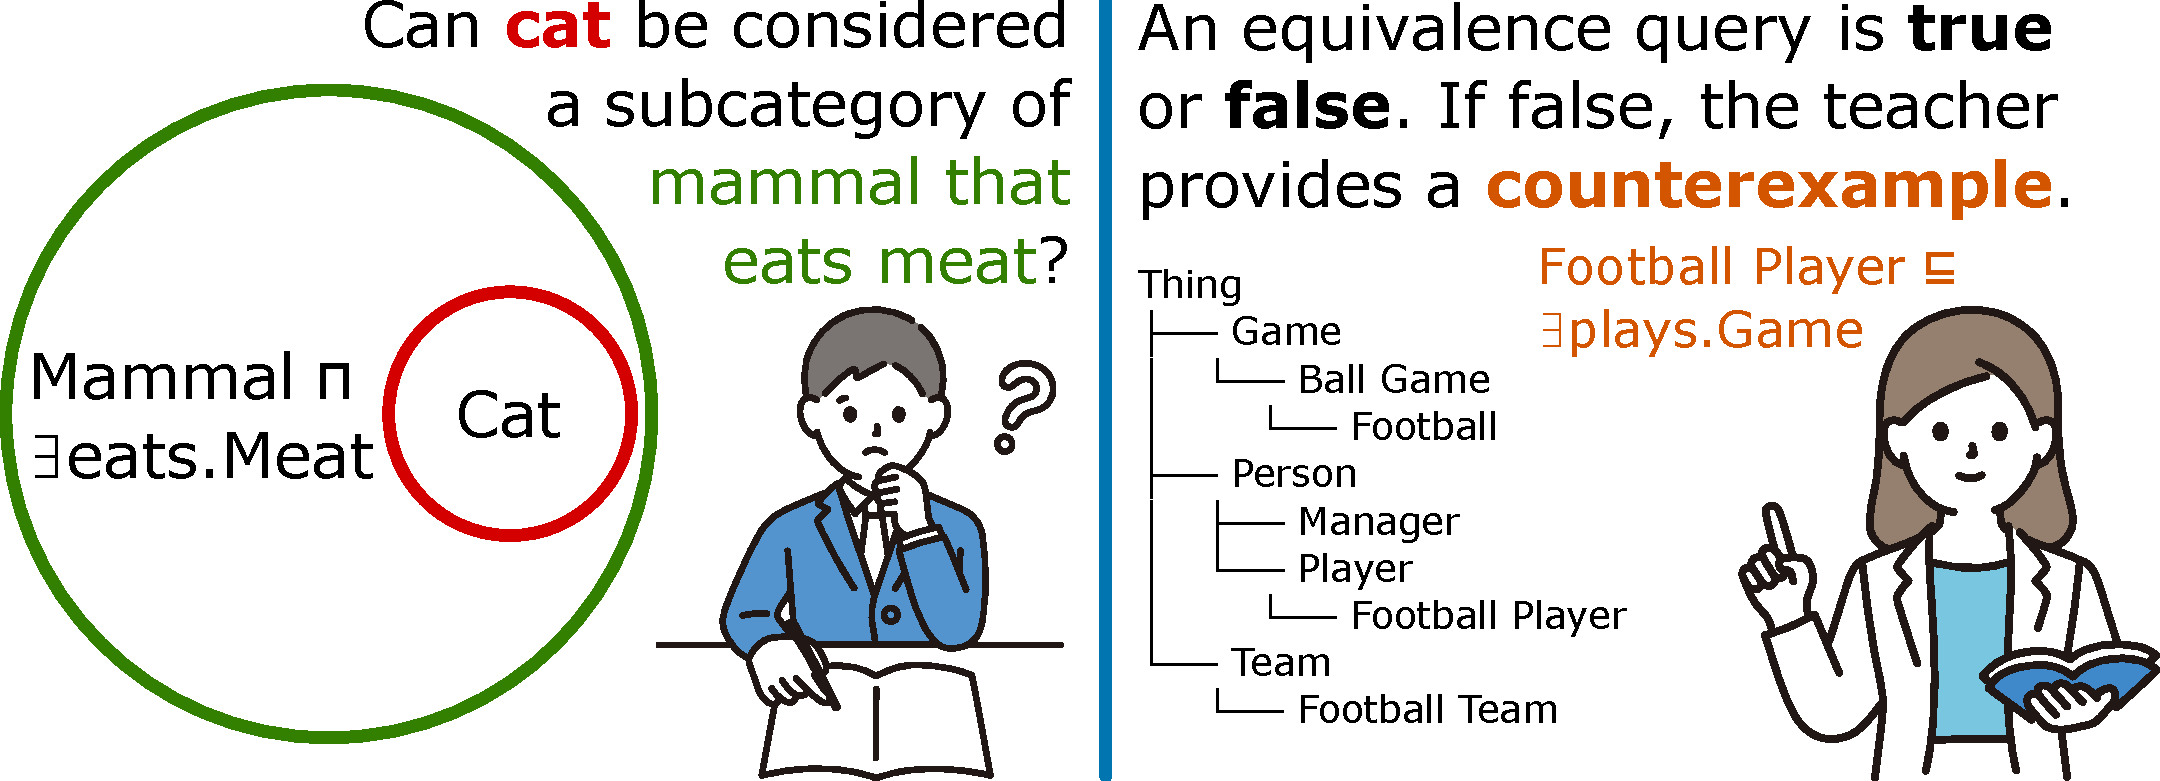
\includegraphics[width=0.7\textwidth]{figures/queries-example}
        \caption{Example of membership and equivalence queries}
        \label{}
    \end{figure}

    We want to use \alert{Large Language Models} (LLMs) as teachers in the \alert{Angluin}'s exact learning framework \ccite{DBLP:journals/ml/Angluin87}.

\end{frame}
%\\\\\\\\\\\\\\\\\\\\\

%\\\\\\\\\\\\\\\\\\\\\
\begin{frame}[c]{Motivation}
    Some motivations for our work:
    %
    \vfill
    %
    \begin{itemize}
        \item to the best of our knowledge, the only implementation of the Angluin's exact learning framework uses a \alert{synthetic teacher} \ccite{DBLP:conf/kr/DuarteKO18}
        %
        \item ontology construction is a costly and time-consuming task that requires domain experts
        %
        \item arguably, a boring and repetitive task for humans
        %
        \item with LLMs as teachers, we can \alert{automate} the process of ontology construction
        %
        \item with Angluin's framework, we build ontologies in a systematic way
        %
    \end{itemize}
\end{frame}
%\\\\\\\\\\\\\\\\\\\\\

%\\\\\\\\\\\\\\\\\\\\\
\begin{frame}{Some state of the art (optional)}

    Provide relevant information about the state of the art / related works here, possibly with references

\end{frame}
%\\\\\\\\\\\\\\\\\\\\\

%\\\\\\\\\\\\\\\\\\\\\
\begin{frame}{Contribution of the paper}

\begin{block}{Explicitly state the contributions of the paper}
    \begin{itemize}
        \item contribution 1
        \item contribution 2
    \end{itemize}
\end{block}

\end{frame}
%\\\\\\\\\\\\\\\\\\\\\

%===============================================================================
\section{Theory / modelling / design}
%===============================================================================

%\\\\\\\\\\\\\\\\\\\\\
\begin{frame}%[allowframebreaks]
\frametitle{Theory / modelling / design}

    Provide 2-3 slides discussing the Theory / modelling / design

\end{frame}
%\\\\\\\\\\\\\\\\\\\\\

\section{Case study / Experiments / Results}

%\\\\\\\\\\\\\\\\\\\\\
\begin{frame}%[allowframebreaks]
\frametitle{Case study / Experiments / Results}

    Provide 2-3 slides discussing the Case study / Experiments / Results of the paper

\end{frame}
%\\\\\\\\\\\\\\\\\\\\\

\section{Conclusions \& future works}

%\\\\\\\\\\\\\\\\\\\\\
\begin{frame}%[allowframebreaks]
\frametitle{Conclusions \& future works}

\begin{block}{Summing up}
    Summarise the most relevant contributions of this study:
    %
    \begin{itemize}
        \item conclusion 1
        \item conclusion 2
        \item conclusion 3
    \end{itemize}
\end{block}

\begin{exampleblock}{Future works}
    Sketch some future research directions
    %
    \begin{itemize}
        \item future work 1
        \item future work 2
    \end{itemize}
\end{exampleblock}

(may be split into 2 slides)

\end{frame}
%\\\\\\\\\\\\\\\\\\\\\

%===============================================================================
\section*{}
%===============================================================================
\frame{\titlepage}

%===============================================================================
\section*{\bibname}
%===============================================================================

\setbeamertemplate{page number in head/foot}{}
%\\\\\\\\\\\\\\\\\\\\\
\begin{frame}[t,allowframebreaks,noframenumbering]\frametitle{\refname}
% \begin{frame}[c]\frametitle{\refname}
	\footnotesize
%	\scriptsize
    \bibliographystyle{apalike-AMS}
    % \bibliographystyle{plain}
	\bibliography{magnini-ecai-2025-talk}
\end{frame}
%\\\\\\\\\\\\\\\\\\\\\

%%%%%%%%%%%%%%%%%%%%%%%%%%%%%%%%%%%%%%%%%%%%%%%%%%%%%%%%%%%%%%%%%%%%%%%%%%%%%%%%
\end{document}
%%%%%%%%%%%%%%%%%%%%%%%%%%%%%%%%%%%%%%%%%%%%%%%%%%%%%%%%%%%%%%%%%%%%%%%%%%%%%%%%
